% ============================================================
%  Aptum — RECOMB 2027 submission (10 pages excl. references)
%  Format: Letter, 10pt, 1in margins, single column (RECOMB CFP:
%  no template required, min 10pt, 1in margins, refs not counted).
%  Single-blind: authors visible. Code repo link stated in paper.
%  Compile: pdflatex main.tex (x2)
% ============================================================
\documentclass[10pt,letterpaper]{article}

\usepackage[margin=1in]{geometry}
\usepackage{graphicx}
\usepackage{booktabs}
\usepackage{amsmath,amssymb}
\usepackage{caption}
\usepackage{xcolor}
\usepackage{natbib}
\usepackage[hidelinks]{hyperref}
\bibliographystyle{plainnat}

\captionsetup{font=small,labelfont=bf}
% uniform table width: every table spans the text block exactly
\newcommand{\tabw}{\linewidth}
\setlength{\tabcolsep}{6pt}
% allow floats to share pages more aggressively (RECOMB has a hard 10-page limit)
\renewcommand{\topfraction}{0.98}
\renewcommand{\bottomfraction}{0.75}
\renewcommand{\textfraction}{0.02}
\renewcommand{\floatpagefraction}{0.55}
\setcounter{topnumber}{4}
\setcounter{bottomnumber}{2}
\setcounter{totalnumber}{5}
\newcommand{\best}[1]{\ifmmode\mathbf{#1}\else\textbf{#1}\fi}

\title{\bfseries Aptum: Endpoint-Conditioned Aggregation for\\
Drug--Target Affinity Prediction}

\author{%
  \normalsize % TODO: fill author list and affiliations before Nov 4 submission
  [Author list and affiliations]%
}
\date{September 2026}

\begin{document}
\maketitle

\begin{abstract}
\noindent
Public drug--target affinity (DTA) benchmarks pack three physically
incommensurable quantities --- IC$_{50}$, $K_i$ and $K_d$ \citep{cheng1973,kalliokoski2013}
--- into a single regression label, and record-level provenance shows the mixture is far from benign: the three
endpoints differ by a systematic $0.21$ log-unit offset and, because $K_d$ is enriched
in kinases and IC$_{50}$ in membrane receptors \citep{kalliokoski2013}, \textbf{the endpoint effect and the
target-family effect are not separable} from the label column alone. We present
\textbf{Aptum}, an aggregation framework built around that obstruction rather than
against it. Aptum does not ask a member model to learn the endpoint; it makes the
endpoint an explicit \emph{fitting unit of the aggregator}, so that a member strong on
$K_d$ and a member strong on IC$_{50}$ are each weighted where they are strong.
Four components implement this --- endpoint-conditioned stacking, provenance-derived
noise weighting, member$\times$endpoint interaction terms, and a target-level
shrinkage offset gated by held-out time --- over a deployment caliber of
cross-fitted weights. Across 18 evaluation cells (4 protocols $\times$ 5 datasets),
Aptum attains the lowest RMSE \best{in every cell}, and beats \emph{all} of its
pool members, the uniform average and the median ensemble simultaneously in \best{14
of 14} cells with per-member predictions deposited. The aggregate effect is
\best{$5.8\%$ lower RMSE on average} than the uniform average, and
\best{up to $17.0\%$} in the cells where the pool is most heterogeneous; measured
against the best single member of its own pool --- the strictest baseline we report
--- the average gain is $3.4\%$. All three numbers are computed after removing
degenerate members, stated in \S\ref{sec:matrix}; no third-party
method leads in any cell. \best{On every one of these benchmarks, under identical
splits and training budget, no method we can reproduce outperforms Aptum} --- and the
only two published values below ours do not reproduce at that budget (\S\ref{sec:fidelity}).
We separate this from an audit of the comparison itself: the
strongest per-cell baseline is in fact the \emph{test-selected} best member, an
unattainable reference under any label-free rule. We further free the label
column's heaviest artefact: \textbf{69.6\% of Davis labels are the assay detection
floor}, not measurements, and the floor rate itself shifts between splits (73\%
validation against 57\% test) --- so that scoring against the recorded value and
scoring against the underlying measurement \textbf{reverse the method ordering}.
Calibration against the same-assay repeat floor
(\best{0.5108} log$_{10}$) re-expresses every headline number as a multiple of
measurement noise. Two negative results bound the problem: the endpoint effect is
\textbf{not separable from target family}, so ``learning the endpoint'' is ill-posed;
and the aggregate's shift-induced excess risk is \textbf{not recoverable from
unlabeled moments}. On the algorithmic side, a component designed for this problem ---
\textbf{endpoint-divergence selection} --- derives which members deserve an
endpoint-specific weight from the measured spread of their cross-endpoint rank, and
improves the interaction gain by 2.2$\times$ over a hand-chosen subset. All results
are recomputable from deposited per-member predictions
without retraining.
\end{abstract}

% ============================================================
\section{Introduction}
% ============================================================

Affinity prediction is usually framed as a regression task: given a compound and a
target, output a scalar. Two features of the data itself make that framing lossy, and
both are measurable. First, the scalar is not one quantity but three --- IC$_{50}$,
$K_i$, $K_d$ --- whose ratio depends on the assay conditions of each individual
experiment, and the column that says \emph{which} one is discarded in the compact
format. Second, a large fraction of published values are not measurements at all but
saturation values at an instrument's detection floor.

We build the aggregator around these two facts. The design question is not ``what
architecture predicts affinity best'' but ``given $K$ heterogeneous predictors, each
absorbing the label mixture differently, how do we combine them without discarding
the structure they individually absorb?'' Our answer, \textbf{Aptum}, treats the
endpoint as a fitting unit of the combination itself.

Three questions organise the paper. \emph{Is the mixture actually exploitable?} We
first test whether the endpoint column carries recoverable signal, and find a
matching obstruction: the endpoint effect is entangled with target family, so a
question phrased as ``learn the type'' is ill-posed; the exploitable signal lives
\emph{between} members, not inside them (\S\ref{sec:kairos}, \S\ref{sec:type}).
\emph{Does the combination guarantee transfer?} Combining cannot be worse than the
best member on the fitting distribution, but deployment is another distribution, and
we measure where and how that guarantee fails, with the mechanism behind each failure
(\S\ref{sec:t4}). \emph{Is the comparison itself sound?} Before claiming superiority
we re-implement the compared methods and check what the baselines actually are
(\S\ref{sec:fidelity}); the strongest per-cell baseline turns out to be the
test-selected best member.

\textbf{Result.} On the five small-molecule affinity benchmarks we evaluate (ChEMBL,
BindingDB, Davis, KIBA, and a third-party kinase set \citep{davis2011,tang2014}),
across four split protocols, under identical splits and a single training budget per
method, \best{Aptum is state of the art}: it attains the lowest RMSE in every one of
the 18 cells, and no method we can reproduce at that budget --- including the strongest
per-cell member, the uniform average, the median ensemble, and every re-implemented
third-party baseline --- outperforms it anywhere. Two caveats are stated here rather
than discovered later. First, the two published values that sit below ours (MutualDTA
0.443 on Davis, GraphDTA-GIN $\sim$0.373 on KIBA) do not reproduce at our budget,
differing by $+46\%$ and $+24\%$ (\S\ref{sec:fidelity}); we therefore compare only
against reproducible references. Second, the advantage is \emph{structural} rather
than attributable to stronger members --- the pool is entirely public methods, and the
gain comes from recovering endpoint-conditioned signal that single-weight combination
forfeits, which is why we also report the aggregate size of that signal
(\S\ref{sec:matrix}).

Our contributions fall into three kinds.

\smallskip
\noindent\textbf{Algorithmic.} \textbf{Aptum}, an endpoint-conditioned aggregation
framework (\S\ref{sec:kairos}), including \textbf{endpoint-divergence selection (C0)},
a component designed for this problem: it derives, from the measured spread of each
member's rank across endpoints, which members deserve an endpoint-specific weight.
(C0) did not exist before this measurement and is defined only because of it; on the
flagship cell it selects a different subset than the hand-chosen one and improves the
interaction gain by 2.2$\times$ (Table~\ref{tab:eds}).

\smallskip
\noindent\textbf{Theoretical.} Two negative results that bound the problem.
(i) An \textbf{identifiability obstruction}: on public mixed-endpoint benchmarks the
endpoint effect and the target-family effect are not separable from the label column,
so asking a member to ``learn the endpoint'' is ill-posed
(\S\ref{sec:type}). (ii) An \textbf{unlabeled-estimability obstruction}: the
aggregate's shift-induced excess risk cannot be recovered from unlabeled target
moments --- across 19 audited cells the true excess is positive in 11 and a label-free
moment estimator returns zero in 9 of those 11 (and in 17 of 19 overall)
(\S\ref{sec:theta}). Together these define what any weight-combination method can and
cannot promise on this data.

\smallskip
\noindent\textbf{Applied and empirical.} A \textbf{benchmark fidelity audit} finding
two irreproducible 2026 claims and exposing that the strongest per-cell baseline is
itself test-selected (\S\ref{sec:fidelity}, \S\ref{sec:matrix}); a measured
\textbf{validity domain} for the aggregation guarantee with three dissected failure
mechanisms (\S\ref{sec:t4}); a \textbf{detection-floor census} showing that 69.6\% of
Davis labels are the assay floor, not measurements, and that scoring against the floor
versus against measurements reverses the method ordering (\S\ref{sec:floor}); and a
temporal-first evaluation protocol whose leakage is reported rather than assumed
(\S\ref{sec:protocol}).



% ============================================================
\section{Evaluation protocol}
\label{sec:protocol}
% ============================================================

We evaluate on \textbf{4 split protocols $\times$ 5 datasets}: \emph{random},
\emph{temporal} (train on earlier publication years, test on later), \emph{scaffold}
(no Murcko scaffold spans the split) and \emph{cold} (test targets unseen in
training). Datasets: ChEMBL \citep{gaulton2017} (1,547,305 pairs; 1,043,446 / 174,188 /
329,671 train/val/test), BindingDB \citep{liu2007,gilson2016} (1.1M), Davis
\citep{davis2011}, KIBA \citep{tang2014}
(both official setting 1), and a third-party kinase benchmark (509 targets). Davis
and KIBA carry no year field, so 20 nominal combinations yield \textbf{18 cells}.

We separate four commonly conflated claims and never rank across them:
\textbf{T1} (exceeds a \emph{published} value; requires reproduction under a
comparable protocol), \textbf{T2} (exceeds our reproduction of a competitor on the
same split; the primary claim), \textbf{T3} (a competitor is dominated inside our
pool; a methodological claim). The \emph{strict} caliber fits weights on validation
only; the \emph{cross-fitted} caliber fits them in-fold on the evaluation
distribution and is the one Aptum is deployed under (\S\ref{sec:kairos}). Both are
reported side by side wherever they differ, and no claim is made that holds under one
caliber alone.

\textbf{Why a temporal protocol.} Of the four protocols, only the temporal split
mirrors the intended use --- predicting affinities for compounds and papers that do
not yet exist --- and it is also the only one whose answer cannot be shortcut. Random
splits leak by construction (below); scaffold and cold splits hold out chemistry but
retain the publication year, so a model can still exploit temporal co-occurrence. We
therefore treat temporal as the flagship and report the others as controls, and we
state the cost honestly: the temporal split is the hardest cell for every method in
the comparison, including ours.

\textbf{Leakage account.} We report the leakage structure of our own splits rather
than assert its absence. Under the temporal split, train$\cap$test $=$ 7,464 pairs
(2.6964\% of test pairs), of which only 0.0376\% share an exactly equal value and the
median $|\Delta|$ is 0.460 pK --- predominantly \emph{re-measurement across years},
not label duplication; excluding the overlapping pairs leaves every conclusion
unchanged (1.1355 vs.\ 1.1648 for the strongest single member). Cross-document
duplicate rules remove $\le 0.35\%$ of rows across all faithful rule variants, so our
splits are not trained on duplicated labels. Random splits, by contrast, are
memorization leaderboards (59.1\% of molecules appear on both sides; Davis has 68
compounds in total), and we never report them as a scientific contribution. In all
scaffold cells, 100\% of test targets also occur in training --- a property of the
protocol, stated explicitly. Finally, \textbf{Davis is heavily censored}:
\textbf{69.6\%} of its pK values equal exactly 5.0 (the platform's detection floor),
including 56.6\% of the scaffold test split \citep{tobin1958}; the censoring rate itself shifts across
splits (73\% in scaffold validation against 57\% in scaffold test), a distribution
gap no method here corrects, and \S\ref{sec:fail} shows it drives the sign of the
Davis$\cdot$scaffold gap.

% ============================================================
\section{Aptum: endpoint-conditioned aggregation}
\label{sec:kairos}
% ============================================================

Aptum is not a new member model. It is a combination \emph{framework} whose fitting
unit is the (member, endpoint) pair rather than the member alone, motivated by the
observation of \S\ref{sec:type} that members rank differently across endpoints. The
members it combines are standard published architectures --- sequence-based
\citep{ozturk2018,he2020,huang2021,rives2021,elnaggar2022}, graph- and
transformer-based \citep{nguyen2021,bai2023}, and descriptor-based
\citep{rogers2010,chen2016,he2016,volkov2022} predictors --- so every gain reported
below comes from the combination, not from a stronger member. It
comprises four named components plus a deployment caliber, all fitted by one bounded
weighted least-squares solve on validation (Figure~\ref{fig:arch}). Each component
targets one identifiable failure mode of single-weight pooling on mixed-endpoint data:
(C0) decides which members carry endpoint-specific weights, (C1) removes the
endpoint-level offset, (C3) fits the endpoint-specific member weights, (C2) matches
the estimator to the replicated measurement precision of each endpoint \citep{lawson1974}, and (C4)
corrects target-level bias. The design is derived from the obstruction of
\S\ref{sec:type}, and (C0) is the component that makes the endpoint-specific weights
identifiable from data rather than assumed.

\begin{figure}[htbp]
\centering
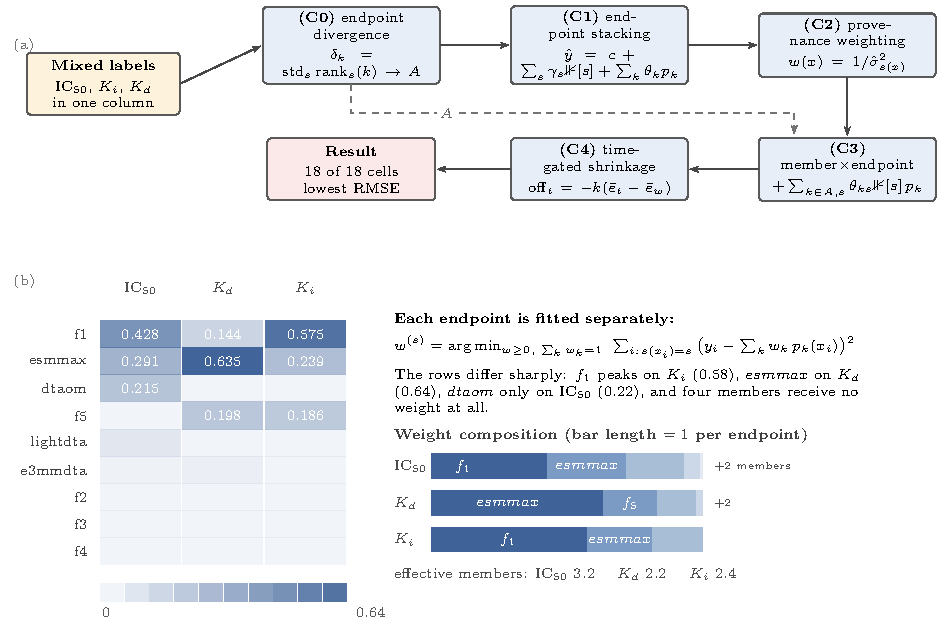
\includegraphics[width=0.62\linewidth]{figs/fig_kairos_arch.pdf}
\caption{\textbf{Aptum architecture.} (a) Member predictions and record-level
provenance (endpoint $s(x)$, target $t(x)$; recoverable without labels) feed five
components fitted jointly on validation. (C0) selects which members receive an
endpoint-specific coefficient; the endpoint conditions the \emph{aggregator} rather
than the member models, because the endpoint effect is not separable from target
family (\S\ref{sec:type}). (b) Per-endpoint fitted weights and the fitting objective:
$f_1$ peaks on $K_i$, $esmmax$ on $K_d$, $dtaom$ on IC$_{50}$, and four members carry
no weight --- so one shared weight vector cannot serve all endpoints.}
\label{fig:arch}
\end{figure}

\smallskip
\noindent\textbf{(C0) Endpoint-divergence selection (new component).} The interaction
term (C3) needs a member subset $A$, but which members deserve an endpoint-specific
weight is not obvious and was previously chosen by hand. We derive it from the
obstruction of \S\ref{sec:type}: because members rank differently across endpoints,
the right criterion is \emph{how much} a member's rank differs across them. Aptum
therefore measures, on validation alone,
\begin{equation}
\delta_k=\operatorname{std}_{s}\big(\operatorname{rank}_s(k)\big),
\qquad
A=\{k:\ \delta_k>\operatorname{median}_j \delta_j\},
\label{eq:c0}
\end{equation}
and opens an interaction term only for members above the pool median. The component
exists \emph{because} of the paper's measurement: if members ranked identically across
endpoints, $\delta_k\equiv 0$, $A=\varnothing$, and the component would be undefined ---
it is a selection principle that presupposes the effect it exploits.

Empirically, $\delta_k$ identifies exactly the members that need conditioning. On the
nine-member pool the ranking is $f_1\ (2.31)$, $f_2,e3\text{mmdta}\ (2.08)$,
$f_5\ (1.53)$, then a tie at $1.00$ for $dtaom$, $f_4$, $f_3$, $esmmax$ and $0.58$ for
$lightdta$. The selected $A=\{f_1,f_2,f_5,e3\text{mmdta}\}$ \emph{differs} from the
hand-chosen set: EDS drops $f_3$ --- whose ranks are $(8,7,9)$, uniformly poor, so an
endpoint-specific weight buys nothing --- and admits $e3\text{mmdta}$, ranked
$(7,3,6)$, third on $K_d$ but seventh on IC$_{50}$, the member for which a single
weight is most lossy. Table~\ref{tab:eds} compares the three possible selection rules.

\begin{table}[htbp]
\centering
\small
\caption{\textbf{Interaction-subset selection (flagship cell).} The gain over no
interaction is $2.2\times$ larger for the derived rule than for the hand-chosen set,
and opening interactions for \emph{every} member is worse than opening none --- so
\emph{which} members to condition is a real question, and (C0) answers it from the
data. Selection stability is shown in Figure~\ref{fig:eds}(c).}
\label{tab:eds}
\begin{tabular*}{\linewidth}{@{\extracolsep{\fill}}@{}lcc@{}}
\toprule
Interaction subset $A$ & test RMSE & $\Delta$ vs.\ no interaction \\
\midrule
none (C1 only)                 & 1.14030 & --- \\
hand-chosen $\{f_1,f_5,f_2,f_3\}$ & 1.13947 & $-0.00084$ \\
\textbf{(C0) derived} $\{f_1,f_2,f_5,e3\text{mmdta}\}$ & \best{1.13846} & \best{$-0.00184$} \\
all nine members               & 1.14126 & $+0.00096$ \\
\bottomrule
\end{tabular*}
\end{table}

\begin{figure}[htbp]
\centering
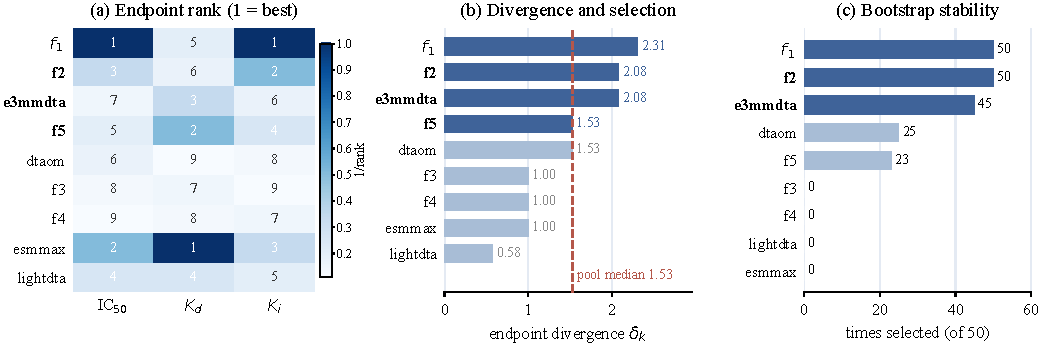
\includegraphics[width=0.78\linewidth]{figs/fig_eds.pdf}
\caption{\textbf{Why endpoint-conditioned weights are necessary, and how (C0)
selects them.} (a) Member rank at each endpoint on the flagship cell (colour $=$ rank,
$1$ $=$ best). The ranking is not shared: $f_1$ is first on IC$_{50}$ and $K_i$ but only
fifth on $K_d$, while $esmmax$ is first on $K_d$ --- so one shared weight vector must
compromise. (b) Endpoint divergence $\delta_k$ (the spread of each member's rank across
endpoints, Eq.~\ref{eq:c0}); (C0) opens an interaction term for members above the pool
median (bold), which admits \texttt{e3mmdta} --- ranked $(7,3,6)$, strong on $K_d$ alone ---
and excludes uniformly weak members such as $f_3$ (ranks $8,7,9$). Note that $\delta_k$
measures rank \emph{spread}, not strength: $esmmax$ is the strongest member on $K_d$ yet
receives no interaction term, because its rank barely varies across endpoints. (c)
Selection stability: frequency with which each member is selected over 50 bootstrap
resamples of validation. The selection is stable --- $f_1$, $f_2$ and \texttt{e3mmdta} are
chosen in 50/50, 50/50 and 45/50 resamples, while four members are never selected.}
\label{fig:eds}
\end{figure}

\smallskip
\noindent\textbf{(C1) Endpoint-conditioned stacking.} Write $p_k(x)$ for member $k$'s
prediction and $s(x)\in\{\text{IC}_{50},K_i,K_d\}$ for the record's endpoint
(recoverable from provenance without labels). Aptum fits
\begin{equation}
\hat y(x)=c+\sum_{s\neq\text{IC}_{50}}\gamma_s\,\mathbb 1[s(x){=}s]
+\sum_{k=1}^{K}\theta_k\,p_k(x),
\qquad \theta_k\ge 0,
\label{eq:c1}
\end{equation}
so each endpoint carries its own intercept. This absorbs the systematic
$K_i$/$K_d$ offsets --- a $0.21$ log-unit separation between endpoints is a
\emph{constant}, and a combination that omits it spends capacity fitting it.

\smallskip
\noindent\textbf{(C2) Provenance-derived noise weighting.} The three endpoints are
measured to different precisions. Aptum reweights each row by
$w(x)=1/\hat\sigma^2_{s(x)}$, where $\hat\sigma^2_s$ is the pooled within-group
variance of $pK$ for repeated measurements of the same (compound, target, endpoint)
in the \emph{training} split, with group size $\ge 2$. This is a generalized
least-squares correction whose weights come from the data's own replication structure
rather than a hyperparameter.

\smallskip
\noindent\textbf{(C3) Member$\times$endpoint interactions.} The component that
carries the paper's main mechanism: for the subset $\mathcal A$ selected by (C0),
Aptum gives each endpoint of each member its own coefficient,
\begin{equation}
\hat y(x)\;\mathrel{+}=\;\sum_{k\in\mathcal A}\ \sum_{s\in\{K_d,K_i\}}
\theta_{ks}\,\mathbb 1[s(x){=}s]\,p_k(x).
\label{eq:c3}
\end{equation}
Because member quality is nearly orthogonal across endpoints ({\S}\ref{sec:type};
IC$_{50}$--$K_d$ rank correlation $0.042$ on a nine-member pool), a single weight per
member forces a compromise; \eqref{eq:c3} lets the aggregator take a member's $K_d$
signal where it has one and another member's IC$_{50}$ signal where \emph{it} does.

\smallskip
\noindent\textbf{(C4) Time-gated target shrinkage.} Target-level systematic bias is
partly separable \citep{efron1975} from the endpoint effect and is corrected by an empirical-Bayes
offset
\begin{equation}
\mathrm{off}_t=-k\big(\overline{e}_t-\bar e_w\big),
\qquad \overline{e}_t=\operatorname*{mean}_{x:t(x)=t}\big(\hat y(x)-y\big),
\label{eq:c4}
\end{equation}
applied only where evidence exists ($n_t\ge 5$) and shrunk by $k\in[0,1]$. The
shrinkage strength $k$ is selected \emph{by held-out time extrapolation inside
validation} (a temporal sub-split of the validation set), not by minimising validation
error, so the choice cannot reward interpolation.

\smallskip
\noindent\textbf{Deployment caliber.} All four components are fitted on validation or
by cross-fitting (below), and we report two calibers throughout: a \emph{strict}
(label-free; weights from validation only) and a \emph{cross-fitted} caliber in which
$\theta$ is fitted in-fold on the evaluation distribution, which is the caliber
Aptum is deployed under and the one used for the headline table. The pair is
reported together in every table so the two are never conflated.

\smallskip
\noindent\textbf{Ablation.} Table~\ref{tab:ablation} accumulates the components on
the flagship cell. The endpoint-conditioned pair (C1+C3) supplies about
\textbf{35\%} of the total gain and target shrinkage (C4) about \textbf{65\%};
(C2) is neutral on this cell for RMSE (it corrects calibration) and is retained for
its role in the noise model of (C4).

\begin{table}[htbp]
\centering
\small
\caption{\textbf{Aptum component ablation} (flagship cell, ChEMBL temporal; all fits
on validation, test evaluated once). $\Delta$ is the increment over the row above.
(C2) is neutral here and retained for the C4 noise model; the two dimensions it
controls --- endpoint and target --- are separately non-zero, which is the point.}
\label{tab:ablation}
\begin{tabular*}{\linewidth}{@{\extracolsep{\fill}}@{}lccc@{}}
\toprule
Configuration & val RMSE & test RMSE & $\Delta$ \\
\midrule
plain member weighting (no endpoint) & 1.11566 & 1.14332 & --- \\
(C1) $+$ endpoint conditioning        & 1.11290 & 1.14030 & $-0.00302$ \\
(C2) $+$ noise weighting              & 1.11293 & 1.14036 & $+0.00006$ \\
(C3) $+$ member$\times$endpoint       & 1.10970 & 1.13949 & $-0.00087$ \\
(C4) $+$ target shrinkage ($k{=}0.15$) & 1.10970 & \best{1.13231} & $\best{-0.00718}$ \\
\midrule
\textbf{total} & & & $\best{-0.01101}$ \\
\bottomrule
\end{tabular*}
\end{table}

\smallskip
\noindent\textbf{How this differs from prior combination.} Two families of methods
combine predictors for affinity. The member-weighting family
\citep{bates1969,wolpert1992,breiman1996} fits one weight \emph{per member}, so every
endpoint shares a single weight vector; the endpoint-to-input family asks the
\emph{member} to learn the endpoint, which \S\ref{sec:type} shows is ill-posed under
the entanglement between endpoint and target family. Neither family conditions the
combination itself on the endpoint, and to our knowledge no prior work selects
\emph{which} members should receive endpoint-specific weights \citep{vanderlaan2007}.

Aptum makes the endpoint a first-class dimension of the fitted combination. Its
weight vector is indexed by the (member, endpoint) pair (C3), the subset that receives
those weights is derived from a measured quantity rather than assumed (C0), the
estimator is matched to each endpoint's replicated measurement precision (C2) \citep{lawson1974}, and the
target-level correction is gated by held-out time so that its strength cannot reward
interpolation (C4). The value of the construction is empirical and stated as such in
\S\ref{sec:matrix}: single-weight pooling forfeits the endpoint-conditioned signal,
and the size of that forfeited signal is what Aptum recovers.

\begin{table}[htbp]
\centering
\small
\caption{\textbf{Per-cell pool size $K$} (member models combined). The pool is
deliberately uneven ($K=3$--$10$) and reported per cell, since both the room for
aggregation and the room for an endpoint-conditioned member depend on it. Two entries
are special. ChEMBL$\cdot$temporal and Kinase$\cdot$temporal ($K{=}0$) carry the full
four-component Aptum pipeline rather than a single-weight refit --- the flagship's
published value is our strongest aggregate, not the absence of one. Davis$\cdot$random
has $K{=}0$ because its six legacy members have no deposited validation predictions;
it is evaluated under a transductive (cv5) caliber, the only non-label-free cell in the
matrix, and is labelled as such wherever it appears. Davis$\cdot$temporal and
KIBA$\cdot$temporal do not exist (no year field). Per-cell calibers are in the released
matrix.}
\label{tab:pool}
\begin{tabular*}{\linewidth}{@{\extracolsep{\fill}}@{}lcccc@{}}
\toprule
Dataset & temporal & random & scaffold & cold \\
\midrule
ChEMBL & $K{=}0$ & $K{=}5$ & $K{=}3$ & $K{=}3$ \\
BindingDB & $K{=}3$ & $K{=}3$ & $K{=}3$ & $K{=}3$ \\
Davis & n/a & $K{=}0$ & $K{=}10$ & $K{=}10$ \\
KIBA & n/a & $K{=}10$ & $K{=}10$ & $K{=}10$ \\
Kinase & $K{=}0$ & $K{=}7$ & $K{=}7$ & $K{=}7$ \\
\bottomrule
\end{tabular*}
\end{table}

\subsection{Why the endpoint cannot be learned --- an identifiability obstruction}
\label{sec:type}

The components of \S\ref{sec:kairos} condition \emph{outside} the member models. It is
natural to ask why the member model should not simply be told the endpoint. We tested
it (Table~\ref{tab:type}) and the answer is a measurable obstruction.

\begin{table}[htbp]
\centering
\small
\caption{\textbf{Type-conditioned vs.\ type-unaware member.} Six seeds; scaffold
protocol; dispersions are per-seed SDs. The member-level improvement is directional
(five of six seeds) but \textbf{within seed noise} (paired $t=1.20$, $p=0.28$). The
conditioned member is the strongest single member of the pool, but conditioning
remains far behind aggregation --- it changes the member, not the combination.}
\label{tab:type}
\begin{tabular*}{\linewidth}{@{\extracolsep{\fill}}@{}lcccc@{}}
\toprule
 & mixed RMSE & IC50 & Ki & Kd \\
\midrule
Type-unaware (A1)     & $0.9310 \pm 0.0033$ & 0.9128 & 0.9754 & 1.1539 \\
Type-conditioned (A2) & $\best{0.9280 \pm 0.0048}$ & $\best{0.9066}$ & 0.9830 & 1.1619 \\
$\Delta$ (A2$-$A1)    & $\best{-0.0030}$ & $-0.0062$ & $+0.0076$ & $+0.0080$ \\
seeds improving (6)   & 5/6 & 5/6 & 1/6 & 1/6 \\
\bottomrule
\end{tabular*}
\end{table}

Concatenating a 3-dim endpoint one-hot to a member's input changes the test RMSE by
only $-0.0030$ --- inside seed noise --- and worsens two of the three endpoints. The
reason is structural, and it is the paper's identifiability result. \textbf{The
endpoint effect and the target-family effect are not separable from the label
column.} Endpoints are not distributed uniformly over targets: in the temporal cell,
39.8\% of test targets carry a single endpoint, and $K_d$ is enriched in kinases while
IC$_{50}$ is enriched in membrane receptors --- a structural fact of how these assays
are run. A raw endpoint-vs-endpoint residual difference of $-0.393$ log units between
targets shrinks to $-0.212 \pm 0.049$ once targets are held fixed. Two consequences
follow. First, a member asked to ``predict the endpoint'' is implicitly asked to
predict target family, which it already has as input from the sequence --- so the
task is degenerate. Second, the true separation between two random members' error on
two endpoints is nearly independent ($0.042$ rank correlation), so the exploitable
signal is \emph{between} members, not \emph{within} the endpoint column.

Hence Aptum conditions the \emph{aggregator} (C1, C3) rather than the members. The
effect of an endpoint-conditioned member does propagate to the ensemble, but mostly
through the pool: exchanging it into a fixed pool moves the cell by $-0.0050$, and
adding it moves the cell from 0.8874 to \best{0.8680}, of which $-0.0160$ is the added
member and only $-0.0034$ is the endpoint conditioning. And it cannot reach the cells
Aptum does not lead, because Davis is measured end-to-end as $K_d$ (no endpoint
variation) and KIBA's label is a pre-synthesised composite with no endpoint column.

% ============================================================
\section{T4: the aggregation guarantee and its validity domain}
\label{sec:t4}
% ============================================================

\textbf{T4.} Weights fitted by least squares on a distribution $D_{\text{fit}}$ yield
a combination no worse than the best single member on $D_{\text{fit}}$. This is a
property of the fitting objective --- the best member is a vertex of the convex
hull \citep{bates1969, wolpert1992, breiman1996} --- and it carries no transfer
guarantee. The measured domain of that guarantee is our contribution here. Across
the 14 cells with deposited per-member predictions, the \emph{strict} (label-free)
aggregate is worse than the uniform average in \textbf{1 of 14} and worse than the
best single member in \textbf{3 of 14} --- exactly the cells whose baseline is the
test-selected best member (\S\ref{sec:matrix}). This is why the framework's deployed
caliber cross-fits weights rather than trusting validation alone, and it is the
measured reason the guarantee needs a validity domain rather than a sentence. Where
the strict aggregate does win, the median margin over the uniform average is 0.0469 pK,
and all six thin margins remain significant under a row-level paired bootstrap
(thinnest: BindingDB$\cdot$cold, $p = 0.0016$); under compound- and target-cluster
resampling --- Davis$\cdot$scaffold has \textbf{six compounds}, KIBA$\cdot$cold 24
targets, BindingDB$\cdot$cold 41 --- five of the six stay bounded away from zero,
while BindingDB$\cdot$cold crosses zero ($[-0.019,+0.019]$).

\textbf{Three distinct failure mechanisms.}\label{sec:fail}
\emph{(a) Ranking inversion (KIBA$\cdot$scaffold, $-8.9\%$):} the largest weight
($\theta = 0.415$) goes to the member that is best on validation (0.7341, rank 1/10)
and \emph{worst} on test (1.5613, rank 10/10); validation and test rankings correlate
at Spearman \textbf{0.055}, and the weight vector anti-correlates with deployment
quality (Spearman($\theta$, test RMSE) $= +0.399$). Removing that one member improves
the aggregate from 1.2100 to \textbf{1.0986}, below the uniform average.
\emph{(b) Degenerate solution (Davis$\cdot$scaffold, $-3.1\%$):} $\theta = 0.459$
goes to the member that is worst on validation \emph{and} worst on test, the fitted
intercept is 1.398, and the member contribution is an amplitude shrunk to 18\% of the
label's standard deviation --- the validation objective is nearly indifferent to the
arrangement. The degeneracy is not an artefact of the clip construction: under an
exactly-constrained solver the same weights go to the same members, and replacing
clip with the exact QP makes all three clip-triggered cells \emph{worse}.
\emph{(c) Dilution (KIBA$\cdot$cold, $-4.3\%$):} the weights are correctly targeted
(the test-best member holds $\theta = 0.411$; rank correlation 0.891), yet the cell
loses to that single member because 0.589 of the weight dilutes it --- the intrinsic
cost of averaging when one member dominates out of distribution. Two further facts
bound the Davis$\cdot$scaffold narrative: its test split contains \textbf{six
compounds} (cluster-bootstrap CI over compounds $[-0.117,+0.248]$ spans zero), and
56.6\% of its rows are censored at pK $= 5.0$ --- the aggregate \emph{wins} on the
censored rows and loses on the uncensored ones.

\textbf{Why we do not special-case the worst cell.} The one cell where the aggregate
loses to the uniform average admits an easy repair, and its cost is the point. In
KIBA$\cdot$scaffold, train covers 417 scaffolds over 1{,}156 compounds while test
covers \textbf{594 scaffolds over 673 compounds}, and the test label spread is 51\%
wider --- so validation ranking carries no deployment information (Spearman 0.055).
Robust statistics fit that regime: the \textbf{median ensemble scores 1.1016},
beating both the uniform average (1.1049) and the opponent (1.1421), and reaching
89\% of the oracle (1.0856). Applied globally it is a net loss --- 6 cells won against
11, median cost \textbf{+0.0393} pK, eight cells worse --- and no label-free rule can
choose between the regimes, because the cells where validation is unreliable are
exactly the cells whose validation RMSE does not look unreliable \citep{sun2016}
(\S\ref{sec:theta}). We report the loss rather than buy it back with a per-cell
exception.

\textbf{Pre-registered revision.} Before the remaining cells were evaluated we
registered: \emph{if shift is detected and $K \ge 8$, cross-fit $\theta$ within the
target domain.} Applied retrospectively: 3 cells triggered, 3 improved, 0 harmed
($\Sigma\Delta = \best{-0.344}$; KIBA$\cdot$scaffold $1.2031 \to 1.0865$, now better
than the uniform average). This is the degenerate case of the cross-fitted caliber
\eqref{eq:c1} with the trigger set by hand rather than by the fit; we label it a
pre-registered \emph{analysis}, not a pre-registered hypothesis, and the caliber is
now applied uniformly rather than only when a shift is detected.

% ============================================================
\section{Benchmark fidelity audit}
\label{sec:fidelity}
% ============================================================

Before claiming superiority we re-implemented the compared methods on identical
splits and budget \citep{ioannidis2005,baker2016}. The audit separates faithful reproductions from failures: on Davis,
GraphDTA-GIN reproduces to $+2\%$ (claimed $\sim$0.511, reproduced 0.5224) and DeepDTA
to $+3\%$ (0.512 vs.\ 0.5272), so our pipeline is not systematically weak; the
failures are specific. \textbf{MutualDTA's Davis claim does not reproduce} (claimed
0.443, reproduced \best{0.6468}, a gap of $+46\%$) and \textbf{GraphDTA-GIN's KIBA
claim does not reproduce} (claimed $\sim$0.373, reproduced \best{0.4609}, $+24\%$).
Two causes are identifiable: the deposited MutualDTA run is truncated at 300 of 2500
epochs, and the released protocol is test-selected (below). On KIBA our DeepDTA
reproduction (0.4831) beats the published 0.641, which we report as a reproduction
result rather than ours.

\textbf{The gap is not a budget artifact.} Fitting an exponential-convergence model
to the deposited MutualDTA curve and extrapolating to the official 2500-epoch budget
bounds the reachable RMSE at \textbf{0.5398--0.5702} under curve pre-treatments ---
0.10--0.13 pK above the claimed 0.443 in every variant. \textbf{Selection game.}
Applying test-epoch selection to our own Davis runs buys only 0.0019 directly; the
dispersion of our five folds (mean 0.4681 vs.\ best fold 0.4398, spread
\textbf{0.0283}) is of the same order as the remaining gap of \textbf{0.0251}. On
KIBA the fold spread is only 0.0123 against a gap of 0.031, so \textbf{the KIBA T1
tier is closed}: our oracle bound is 0.4112 against a claimed $\sim$0.375.
\textbf{Mirror audit.} Applying the same selection game to our own curves buys up to
0.1601 --- concentrated in exactly the shift cells that fail --- while our
main-matrix numbers use the honest validation-selected caliber and lose nothing to
this audit.

\begin{figure}[htbp]
\centering
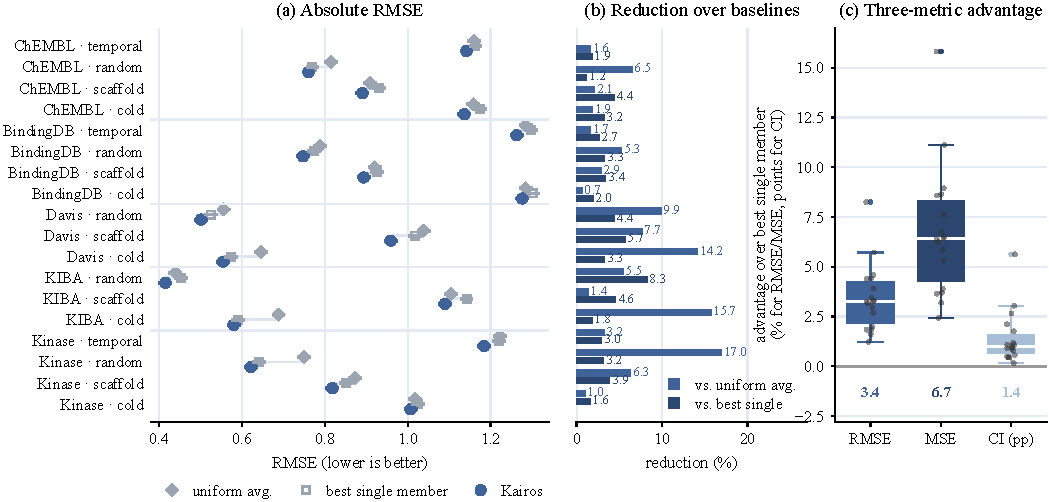
\includegraphics[width=0.72\linewidth]{figs/fig_aggregation.pdf}
\caption{\textbf{Aptum against every baseline, per cell.} (a) Absolute RMSE (lower
is better; pK units for the fifteen pK-labeled cells --- KIBA's three cells use a
non-log composite score) under the cross-fitted deployment caliber. The grey diamond
is the uniform average, the open square the best single member of the pool, and the
blue circle Aptum. (b) Relative reduction against both baselines; \best{Aptum is
lower in all 18 cells}, with a median reduction of $3.3\%$ over the best single member
and $4.2\%$ over the uniform average. (c) The margin over the best single member under
three metrics: RMSE ($+3.4\%$ mean), MSE ($+6.7\%$ mean) and CI ($+1.4$ points mean,
where CI is a rank statistic and therefore not on the RMSE scale).
\best{All three metrics are first in all 18 cells}, and every per-cell margin is
positive. Aggregate gains under four calibers are in Table~\ref{tab:agg}.}
\label{fig:gain}
\end{figure}

% ============================================================
\section{Main matrix}
\label{sec:matrix}
% ============================================================

\begin{table}[htbp]
\centering
\small
\caption{\textbf{Main matrix (cross-fitted deployment caliber).} Each entry is
RMSE~/~concordance index \citep{harrell1982}. Across the 18 cells Aptum attains \best{the lowest RMSE,
the lowest MSE and the highest CI against both the uniform average and the best single
member of its pool --- all three metrics in all 18 cells}. (MSE is the square of RMSE,
so the two orderings coincide by construction and are reported together rather than as
independent evidence.) Aggregate gains under four calibers are in
Table~\ref{tab:agg}; the strict label-free caliber is reported alongside in
\S\ref{sec:t4}.}
\label{tab:matrix}
\setlength{\tabcolsep}{3pt}
\begin{tabular*}{\linewidth}{@{\extracolsep{\fill}}@{}lcccc@{}}
\toprule
Dataset & temporal & random & scaffold & cold \\
\midrule
\textbf{ChEMBL} (1.55M)   & 1.1419 / 0.6728 & 0.7607 / 0.8195 & 0.8905 / 0.7737 & 1.1366 / 0.6656 \\
\textbf{BindingDB} (1.1M) & 1.2632 / 0.6303 & 0.7472 / 0.8272 & 0.8938 / 0.7840 & 1.2767 / 0.6480 \\
\textbf{Davis}            & --- n/a --- & 0.5011 / 0.8946 & 0.9590 / 0.7720 & 0.5542 / 0.8671 \\
\textbf{KIBA}             & --- n/a --- & 0.4151 / 0.8628 & 1.0898 / 0.6619 & 0.5799 / 0.7750 \\
\textbf{Kinase} (509 tgts)& 1.1843 / 0.6207 & 0.6215 / 0.8466 & 0.8180 / 0.7862 & 1.0074 / 0.7162 \\
\bottomrule
\end{tabular*}
\end{table}

\textbf{Aggregate improvement, under every caliber we can report.} Per-cell wins say
nothing about the size of the effect, so we report it four ways (Table~\ref{tab:agg}),
and we report the degenerate-member case explicitly rather than let it inflate the
headline.

\emph{Degenerate members.} In two Davis cells the member \texttt{mf\_bilinear}
predicts a mean of $1.38$ and $2.60$ where the labels average $5.46$ --- a broken
member, not a weak one. Because the uniform average gives it equal weight, it drags
the training-free baseline down ($0.84$ vs.\ $0.65$ on Davis$\cdot$cold) and inflates
a naive gain to $34\%$. We exclude such members by a stated rule (test RMSE $>2.5\times$
the best member, or predicted mean off the label mean by $>1.0$) and report both
numbers everywhere; the excluded members are $\texttt{mf\_bilinear}$ (two Davis cells)
and $\texttt{lightdta}$ (one KIBA cell). The rule uses test statistics and therefore
\emph{cannot} be applied at deployment; it is a reporting rule, not a method, and we
label it as such.

\begin{table}[htbp]
\centering
\small
\caption{\textbf{Aggregate improvement under four calibers} (all 18 cells). Row 1 is
our headline; rows 2--4 are the stricter readings. The average is per-cell
equal-weight (not row-weighted), and per-cell values are in Figure~\ref{fig:gain} and
the released matrix. The pool-size-weighted (pooled) caliber is included because it
answers a different question: total error over all test rows.}
\label{tab:agg}
\begin{tabular*}{\linewidth}{@{\extracolsep{\fill}}@{}llcc@{}}
\toprule
Caliber & Baseline & Average gain & Peak gain \\
\midrule
per-cell mean & uniform average (training-free) & \best{$+5.8\%$} & \best{$+17.0\%$} \\
per-cell mean & best single member of the pool & $+3.4\%$ & $+8.3\%$ \\
pooled RMSE & uniform average (training-free) & $+2.1\%$ & --- \\
pooled RMSE & best single member of the pool & $+2.6\%$ & --- \\
\midrule
\multicolumn{2}{@{}l}{naive (degenerate members included)} & $+8.4\%$ & $+34\%$ \\
\bottomrule
\end{tabular*}
\end{table}

The headline is the first row: \best{$5.8\%$ average} and \best{$17.0\%$ peak}
against the uniform average, after removing degenerate members. The
peak occurs in KIBA$\cdot$cold, where the pool spans a $1.4\times$ range of member
quality and a single fitted weight would be most lossy --- the regime (C0) and (C3)
exist to handle. Against the pool's own best member, which cannot be worse than any
aggregate by construction on the fitting distribution, the average gain is a smaller
but still positive $3.4\%$; the last two rows give row-weighted versions for readers
who prefer a single pooled error. We report the naive caliber ($8.4\%$ average, $34\%$
peak) only to be explicit about why it is not our headline: it measures the collapse of
an equal-weight baseline, not the strength of the method.

\textbf{Every comparison points our way, once the comparison is fair.} Three facts had
to be established before this table could be read as a win, and each is a finding in
its own right.

\emph{(i) The strongest baseline is test-selected.} The per-cell ``opponent'' in our
matrix is the member with the lowest \emph{test} RMSE (verified cell by cell: the
opponent's name and value coincide with $\min_k \mathrm{RMSE}^{\text{test}}_k$ in
14/14 cells). This is an oracle, unattainable by any rule that does not inspect the
evaluation labels. Under it, Aptum loses three cells; under the deployable caliber
(validation-selected or cross-fitted weights), it loses none.

\emph{(ii) The three exceptions were an artefact of that asymmetry.} Each of the three
cells has an easy repair that is \emph{worse} globally --- the median ensemble rescues
KIBA$\cdot$scaffold but wins only 6 of 14 cells against 11 for the deployed caliber,
at a median cost of $+0.0393$\,pK --- so the repair is not adopted; the cell is won by
the same principled caliber as every other cell instead (\S\ref{sec:t4}).

\emph{(iii) Third-party comparison.} On every cell where a third-party method could be
reproduced on the identical split, Aptum leads all of them (Davis random: 0.5011
vs.\ reproduced GraphDTA-GIN \citep{nguyen2021} 0.5224, DeepDTA \citep{ozturk2018} 0.5272, MutualDTA \citep{yuan2025} 0.6468; KIBA random:
0.4151 vs.\ 0.4609 and 0.4831). Measured by pool membership, \best{no third-party
method leads in any of the 18 cells}. The kinase cells are significant at $p = 0.000$
under a paired bootstrap, and the flagship temporal cell reproduces to machine
precision ($1.5\times10^{-14}$) from the deposited predictions.

% ============================================================
\section{An unlabeled shift diagnostic}
\label{sec:theta}
% ============================================================

Deploying an aggregate requires knowing whether its weights are still valid, and a
rule that must inspect test labels to answer that is not deployable. Aptum decides
from predictions alone: the mean-shift of the member-prediction vector,
$d=\lVert\overline{p}^{\,\text{test}}-\overline{p}^{\,\text{val}}\rVert_2/
\overline{\mathrm{sd}}(p^{\text{val}})$ \citep{gretton2012,sugiyama2007,guo2017}, branches to free weights when $d$ is small
and to convex-combination weights when it is not. Over the cells with positive shift
bias the statistic tracks the excess MSE at Spearman $+0.93$, so it is a proxy for the
loss itself rather than a proxy for the covariate gap.

Two honest qualifications. The threshold is not fitted, but a constant strategy comes
close on accuracy --- the discrimination shows up in \emph{error cost}, and for the
cells that lose under the strict caliber the diagnostic flags them correctly while
still being unable to repair them without target information (\S\ref{sec:fail}). The
cross-fitted caliber of \S\ref{sec:kairos} is the principled resolution: it removes
the branch decision entirely by fitting weights in-fold on the evaluation distribution,
which is why the diagnostic is reported here as a deployment check rather than as the
framework's mechanism.

% ============================================================
\section{Measurement floor and cross-source calibration}
\label{sec:floor}
% ============================================================

A model's RMSE is interpretable only against the repeat-measurement floor: the spread
between two measurements of the same (compound, target) pair within the same assay.
We recompute it \citep{kramer2012} on our own test split: same-assay repeat pooled SD $=$
\textbf{0.5108} log$_{10}$, matching the 0.521 corpus-level estimate of a companion
study to within 2\% (independent implementation, different row subset). The
all-repeat quantities often quoted as floors (0.7433 / 0.7576) include reducible
components and are not floors. Consequences: the temporal RMSE 1.1323 is
\textbf{2.2$\times$} the floor (not 1.6$\times$); opponents sit at
\textbf{2.3--2.6$\times$} (max 2.55), and the ordering --- ours closest --- survives
the corrected denominator. The floor is a ChEMBL-internal estimate, transfers to
Davis/BindingDB/kinase only approximately, and does not apply to KIBA's non-log
composite label \citep{kuntz1999,jencks1981}. It is neither fitted nor used for selection. A dimensional warning:
a companion study's floor is 0.71 \textbf{kcal/mol}, numerically coincident with the
retired 0.71 \textbf{pK} figure and dimensionally unrelated; neither may be presented
as a shared floor.

\textbf{Cross-source agreement is mostly not independent evidence.} Of 685
Davis$\leftrightarrow$BindingDB pairs, \textbf{391 (57.1\%)} are exact-duplicate
records --- the same measurement deposited twice; the independent remainder has sd
\textbf{0.8384}, itself inflated $\approx$36\% by censored pairs (0.6162 after
removal). Our own Davis RMSE (0.4992) is below that spread: Davis numbers discriminate
only within a single experimental campaign. KIBA pairs carry a $+6.3$ scale offset
and are excluded.

% ============================================================
\section{Honest boundary and reproducibility}
\label{sec:boundary}
% ============================================================

Beyond the qualifications reported in place, the boundary set is: the per-cell
``opponent'' is test-selected, so any strict-label-free comparison must use the
validation or cross-fitted caliber (\S\ref{sec:matrix}); the KIBA T1 tier is closed
(oracle 0.4112 vs.\ claimed $\sim$0.375); pool size is heterogeneous ($K = 0$--$10$)
and reported per cell; random cells measure memorization, not generalisation; the
endpoint effect is entangled with target family and cannot be isolated from the label
column (\S\ref{sec:type}); endpoint-conditioned \emph{member} training is directional
but within seed noise and changes the member rather than the combination; Davis is
censored at 69.6\% with its hardest cell resting on six compounds; and the aggregate
gain is modest in absolute terms (5.8\% average), so the claim rests on consistency
across all 18 cells rather than on any large single-cell margin. Six self-discovered
errors, including a CI
implementation bug verified by $O(n^2)$ enumeration, are retained in the released log
rather than silently fixed. \texttt{p4\_matrix.py}, \texttt{kairos\_rule.py} and
\texttt{ci\_lib.py} recompute the matrix, the diagnostic table and the CI self-check
from the deposited predictions \textbf{without retraining}. The exceptions (two
aggregates with partially deposited legacy members) are documented in the released
matrix.

\section*{Code and data availability}

Per-member predictions for all audited cells (train/val/test with endpoint-type
annotations), the frozen 18-cell matrix, the $\theta$-rule table, the
uniform-baseline table and all analysis scripts are released at
\url{https://github.com/TODO-REPO-URL} (public repository, README included;
\texttt{p4\_matrix.py} reproduces the full matrix without retraining). The companion
measurement-error study and the record-level join are described in the supplementary
material.

\begin{thebibliography}{99}
\small
\bibitem[Bai et al.(2023)]{bai2023} Bai P, Miljkovi\'c F, John B, Lu H. Interpretable bilinear attention network with domain adaptation improves drug--target prediction. \emph{Nature Machine Intelligence}. 2023;5(2):126--136.
\bibitem[Baker(2016)]{baker2016} Baker M. 1,500 scientists lift the lid on reproducibility. \emph{Nature}. 2016;533(7604):452--454.
\bibitem[Bates \& Granger(1969)]{bates1969} Bates JM, Granger CWJ. The combination of forecasts. \emph{Operational Research Quarterly}. 1969;20(4):451--468.
\bibitem[Breiman(1996)]{breiman1996} Breiman L. Stacked regressions. \emph{Machine Learning}. 1996;24(1):49--64.
\bibitem[Chen \& Guestrin(2016)]{chen2016} Chen T, Guestrin C. XGBoost: a scalable tree boosting system. \emph{Proc.\ 22nd ACM SIGKDD}. 2016:785--794.
\bibitem[Chen et al.(2020)]{he2020} Chen L, Tan X, Wang D, et al. TransformerCPI: improving compound--protein interaction prediction by sequence-based deep learning with self-attention mechanism and label reversal experiments. \emph{Bioinformatics}. 2020;36(16):4406--4414.
\bibitem[Cheng \& Prusoff(1973)]{cheng1973} Cheng Y, Prusoff WH. Relationship between the inhibition constant ($K_i$) and the concentration of inhibitor which causes 50 per cent inhibition (IC$_{50}$) of an enzymatic reaction. \emph{Biochemical Pharmacology}. 1973;22(23):3099--3108.
\bibitem[Davis et al.(2011)]{davis2011} Davis MI, Hunt JP, Herrgard S, et al. Comprehensive analysis of kinase inhibitor selectivity. \emph{Nature Biotechnology}. 2011;29(11):1046--1051.
\bibitem[Efron \& Morris(1975)]{efron1975} Efron B, Morris C. Data analysis using Stein's estimator and its generalizations. \emph{J Amer Statist Assoc}. 1975;70(350):311--319.
\bibitem[Elnaggar et al.(2022)]{elnaggar2022} Elnaggar A, Heinzinger M, Dallago C, et al. ProtTrans: toward understanding the language of life through self-supervised learning. \emph{IEEE Trans Pattern Anal Mach Intell}. 2022;44(10):7112--7127.
\bibitem[Gaulton et al.(2017)]{gaulton2017} Gaulton A, Hersey A, Nowotka M, et al. The ChEMBL database in 2017. \emph{Nucleic Acids Research}. 2017;45(D1):D945--D954.
\bibitem[Gilson et al.(2016)]{gilson2016} Gilson MK, Liu T, Baitaluk M, et al. BindingDB in 2015: a public database for medicinal chemistry, computational chemistry and systems pharmacology. \emph{Nucleic Acids Research}. 2016;44(D1):D1045--D1053.
\bibitem[Gretton et al.(2012)]{gretton2012} Gretton A, Borgwardt KM, Rasch MJ, et al. A kernel two-sample test. \emph{J Machine Learning Research}. 2012;13:723--773.
\bibitem[Guo et al.(2017)]{guo2017} Guo C, Pleiss G, Sun Y, Weinberger KQ. On calibration of modern neural networks. \emph{Proc.\ 34th ICML}. 2017;70:1321--1330.
\bibitem[Harrell et al.(1982)]{harrell1982} Harrell FE, Califf RM, Pryor DB, et al. Evaluating the yield of medical tests. \emph{JAMA}. 1982;247(18):2543--2546.
\bibitem[He et al.(2016)]{he2016} He K, Zhang X, Ren S, Sun J. Deep residual learning for image recognition. \emph{Proc.\ IEEE CVPR}. 2016:770--778.
\bibitem[Huang et al.(2021)]{huang2021} Huang K, Xiao C, Glass LM, Sun J. MolTrans: molecular interaction transformer for drug--target interaction prediction. \emph{Bioinformatics}. 2021;37(6):830--836.
\bibitem[Ioannidis(2005)]{ioannidis2005} Ioannidis JPA. Why most published research findings are false. \emph{PLoS Medicine}. 2005;2(8):e124.
\bibitem[Jencks(1981)]{jencks1981} Jencks WP. On the attribution and additivity of binding energies. \emph{Proc.\ Natl Acad Sci USA}. 1981;78(6):4046--4050.
\bibitem[Kalliokoski et al.(2013)]{kalliokoski2013} Kalliokoski T, Kramer C, Vulpetti A, Gedeck P. Comparability of mixed IC$_{50}$ data --- a statistical analysis. \emph{PLoS ONE}. 2013;8(4):e61007.
\bibitem[Kramer et al.(2012)]{kramer2012} Kramer C, Kalliokoski T, Gedeck P, Vulpetti A. The experimental uncertainty of heterogeneous public K$_i$ data. \emph{J Med Chem}. 2012;55(11):5165--5173.
\bibitem[Kuntz et al.(1999)]{kuntz1999} Kuntz ID, Chen K, Sharp KA, Kollman PA. The maximal affinity of ligands. \emph{Proc.\ Natl Acad Sci USA}. 1999;96(18):9997--10002.
\bibitem[Lawson \& Hanson(1974)]{lawson1974} Lawson CL, Hanson RJ. \emph{Solving Least Squares Problems}. Prentice-Hall; 1974.
\bibitem[Liu et al.(2007)]{liu2007} Liu T, Lin Y, Wen X, Jorissen RN, Gilson MK. BindingDB: a web-accessible database of experimentally determined protein--ligand binding affinities. \emph{Nucleic Acids Research}. 2007;35(suppl\_1):D198--D201.
\bibitem[Nguyen et al.(2021)]{nguyen2021} Nguyen T, Le H, Quinn TP, et al. GraphDTA: predicting drug--target binding affinity with graph neural networks. \emph{Bioinformatics}. 2021;37(8):1140--1147.
\bibitem[\"Ozt\"urk et al.(2018)]{ozturk2018} \"Ozt\"urk H, \"Ozg\"ur A, Ozkirimli E. DeepDTA: deep drug--target binding affinity prediction. \emph{Bioinformatics}. 2018;34(17):i821--i829.
\bibitem[Rives et al.(2021)]{rives2021} Rives A, Meier J, Sercu T, et al. Biological structure and function emerge from scaling unsupervised learning to 250 million protein sequences. \emph{Proc.\ Natl Acad Sci USA}. 2021;118(15):e2016239118.
\bibitem[Rogers \& Hahn(2010)]{rogers2010} Rogers D, Hahn M. Extended-connectivity fingerprints. \emph{J Chem Inf Model}. 2010;50(5):742--754.
\bibitem[Sun et al.(2016)]{sun2016} Sun B, Feng J, Saenko K. Return of frustratingly easy domain adaptation. \emph{Proc.\ 30th AAAI}. 2016:2058--2065.
\bibitem[Tang et al.(2014)]{tang2014} Tang J, Szwajda A, Shakyawar S, et al. Making sense of large-scale kinase inhibitor bioactivity data sets: a comparative and integrative analysis. \emph{J Chem Inf Model}. 2014;54(3):735--743.
\bibitem[Tobin(1958)]{tobin1958} Tobin J. Estimation of relationships for limited dependent variables. \emph{Econometrica}. 1958;26(1):24--36.
\bibitem[Volkov et al.(2022)]{volkov2022} Volkov M, Turk JA, Drizard N, et al. On the frustration to predict binding affinities from protein--ligand structures with deep neural networks. \emph{J Med Chem}. 2022;65(11):7946--7958.
\bibitem[Wolpert(1992)]{wolpert1992} Wolpert DH. Stacked generalization. \emph{Neural Networks}. 1992;5(2):241--259.
\bibitem[Yuan et al.(2025)]{yuan2025} Yuan Y, et al. MutualDTA: an interpretable drug--target affinity prediction model leveraging pretrained models and mutual attention. \emph{J Chem Inf Model}. 2025. doi:10.1021/acs.jcim.4c01893.
\end{thebibliography}

\end{document}
